\documentclass[11pt,a4paper]{article}

\usepackage[utf8]{inputenc}
\usepackage[T1]{fontenc}
\usepackage[margin=2.5cm]{geometry}
\usepackage{graphicx}      % images (paths with spaces work in LaTeX 2019+)
\usepackage{float}
\usepackage{amsmath}
\usepackage{booktabs}
\usepackage{cite}          % numeric citations: [1], [1,2], [1--3]
\usepackage[hidelinks]{hyperref}

\title{HMS Harmful Brain Activity Classification}
\author{}
\date{\today}

\begin{document}

\maketitle

% ======================================================================
\section{Background}
% ======================================================================
% Example citation: Seizures are associated with brain injury~\cite{ref1}.



% ======================================================================
\section{Main}
% ======================================================================

% ----------------------------------------------------------------------
\subsection{Phase 1: What is the data}
% ----------------------------------------------------------------------

\subsubsection{Exercise 1: Labels}


\subsubsection{Exercise 2: Signals}


\subsubsection{Exercise 3: Features and patient-grouped cross-validation}


% ----------------------------------------------------------------------
\subsection{Phase 2: Final model}
% ----------------------------------------------------------------------

\subsubsection{Step 0: Template submission}


\subsubsection{Step 1: Class-prior baseline and KL metric}


\subsubsection{Step 2: Phase-1 features with gradient-boosted trees}


\subsubsection{Step 3: Using vote counts}


\subsubsection{Step 4: Evaluation}


\subsubsection{Step 5: Final submission}


% ----------------------------------------------------------------------
% Sample figure (reference for how to include an output image)
% ----------------------------------------------------------------------
\begin{figure}[H]
    \centering
    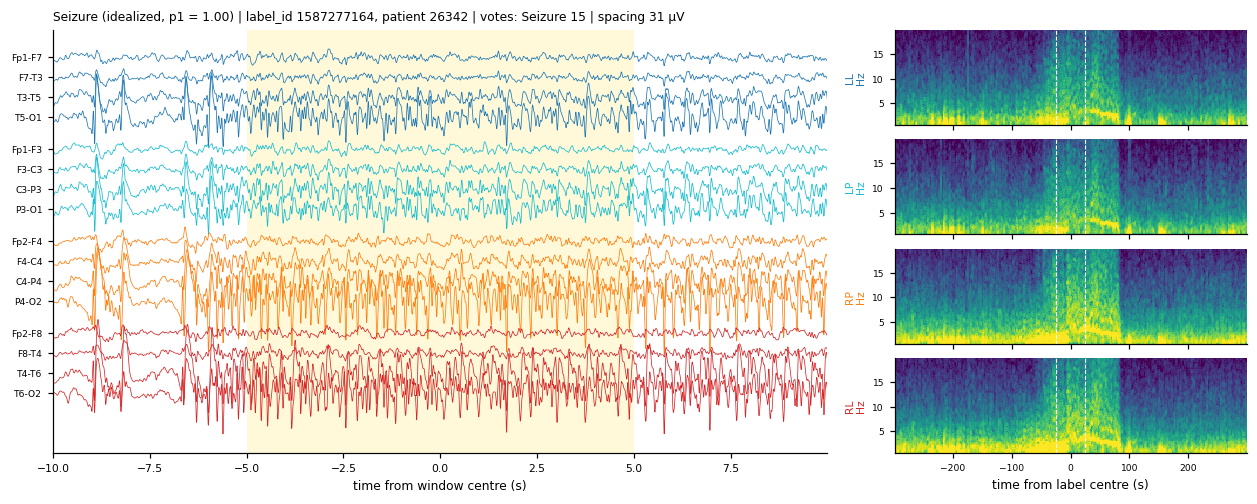
\includegraphics[width=0.9\textwidth]{phase 1/outputs_02/example_Seizure_1587277164.png}
    \caption{Example of a high-agreement Seizure window (placeholder caption).}
    \label{fig:example_seizure}
\end{figure}
% Refer to it in text with: Figure~\ref{fig:example_seizure}


% ======================================================================
\section{Conclusion}
% ======================================================================



% ======================================================================
% References (numbered in order of citation, shown as [1], [2], ...)
% Add entries to bibliography.bib and cite them with \cite{key}.
% ======================================================================
\bibliographystyle{ieeetr}
\bibliography{bibliography}

\end{document}
